\section{Технический проект}

\subsection{Общая характеристика организации решения задачи}

Система построена по схеме <<клиент -- сервер>>. Сервер на Node.js принимает HTTP-запросы: проверяет логин и пароль, выдаёт и проверяет JWT, выполняет запросы к PostgreSQL, собирает ответы социальной ленты в JSON и отдаёт их клиенту. Статические файлы интерфейса (HTML, CSS, JavaScript, ресурсы) отдаются из каталога фронтенда тем же процессом. Если приходит GET по пути, для которого нет отдельного обработчика, сервер отдаёт главную HTML-страницу клиента; маршрутизация внутри приложения дальше выполняется на стороне браузера (одностраничное приложение).

Условно выделяются три уровня:
\begin{enumerate}
	\item Клиент: работа с DOM, сценарии с суффиксом <<.module.js>>, локальное хранилище браузера, построение графиков с помощью Chart.js.
	\item Сервер приложения: маршруты Express, проверка входных данных, ограничение числа запросов на регистрацию и вход.
	\item Данные: таблицы PostgreSQL, доступ через пул соединений библиотеки pg.
\end{enumerate}

После успешного входа клиент в последующих запросах к защищённым URL передаёт JWT в заголовке Authorization. Обработчик маршрута извлекает из токена userId и username и подставляет их в объект запроса. Дополнительные данные пользователя (например, настройки экранов, сохранённые на клиенте) синхронизируются с таблицей user\_storage.

На рисунке~\ref{fig:componentinteraction} показана общая схема взаимодействия компонентов развёрнутой системы: авторизованный пользователь работает через браузер с одностраничным приложением; запросы к REST API и раздача статики выполняются сервером Node.js\,/\,Express; персистентные данные учётных записей, профиля, пользовательского хранилища и социальной ленты хранятся в PostgreSQL; справочные JSON-файлы и библиотека Chart.js подгружаются из статического каталога фронтенда (тот же HTTP-сервер).

\begin{figure}[H]
	\centering
	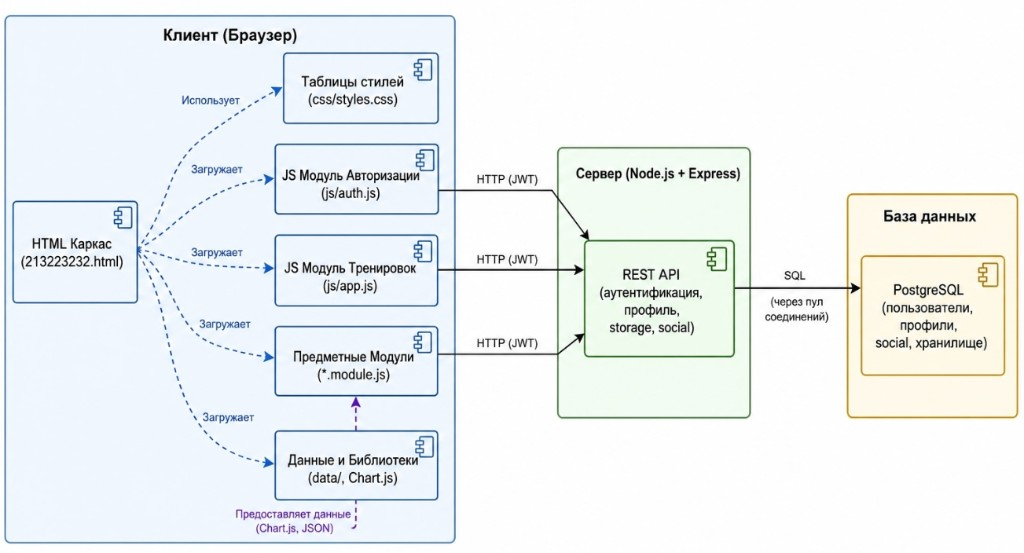
\includegraphics[width=0.98\textwidth]{images/component_interaction}
	\caption{Диаграмма компонентов программно-информационной системы Fitness Life}
	\label{fig:componentinteraction}
\end{figure}

\subsection{Обоснование выбора технологии проектирования}

Стек выбирался из требований задания: нужны реляционная БД с явной схемой, REST API, сервер на JavaScript и возможность отдать готовый статический фронтенд без обязательной сборки через отдельный бандлер.

\subsection{Структура клиентской части}

В клиентской части проекта выделяются следующие основные файлы:
\begin{itemize}
	\item \texttt{213223232.html} -- основная HTML-страница;
	\item \texttt{css/styles.css} -- таблица стилей приложения;
	\item \texttt{js/auth.js} -- клиентский слой авторизации и подготовки состояния;
	\item \texttt{js/app.js} -- основной модуль тренировочного интерфейса;
	\item \texttt{modules/profile.module.js} -- модуль профиля;
	\item \texttt{modules/nutrition.module.js} -- модуль питания;
	\item \texttt{modules/psychology.module.js} -- модуль психологической поддержки;
	\item \texttt{modules/social.module.js} -- модуль социальной ленты;
	\item \texttt{modules/avatar.module.js} -- модуль аватара;
	\item \texttt{data/mental-advice.json} -- данные для раздела поддержки;
	\item \texttt{js/vendor/chart.umd.min.js} -- локальная версия Chart.js.
\end{itemize}

Файловая декомпозиция клиента соответствует принципу единственной ответственности: авторизация отделена от тренировочной логики, а предметные разделы (профиль, лента, питание и др.) вынесены в подключаемые модули. Такой подход облегчает сопровождение -- правки в социальной ленте не должны затрагивать алгоритмы построения графиков -- и отражает зрелую практику организации кода в браузере даже при отказе от тяжёлых SPA-фреймворков в пользу <<склеивания>> логики вручную.

Модуль \texttt{avatar.module.js} на клиенте пересчитывает опыт и уровень персонажа, опираясь на данные тренировок (\texttt{app.js}, история подходов), дневника питания (\texttt{nutrition}) и чекинов раздела <<Поддержка>> (\texttt{psychology}); социальная лента в этот расчёт не входит.

\subsection{Организация HTML-страницы}

Основная HTML-страница содержит два ключевых корневых блока: \texttt{authRoot} и \texttt{appRoot}. Первый используется для отображения формы авторизации и регистрации. Второй содержит основной интерфейс и по умолчанию скрывается до завершения входа пользователя.

Внутри \texttt{appRoot} находится верхняя панель: кнопка профиля (открывает отдельную вкладку \texttt{profile-tab}), виртуальный аватар пользователя (\texttt{virtualAvatarMount}), имя пользователя и ряд вкладок \texttt{data-tab}.

Тренировочная вкладка содержит трёхколоночную разметку. Остальные предметные разделы имеют контейнеры \texttt{\#nutrition-tab}, \texttt{\#social-tab}, \texttt{\#psychology-tab}, \texttt{\#avatar-tab}, куда через \texttt{AppModules.*.render()} монтируются модули. Внизу корня приложения описаны элементы общих модальных окон (\texttt{\#modal}, \texttt{\#confirmModal}, \texttt{\#alertModal}) для единого визуального поведения.

\subsection{Вкладочный интерфейс}

Вкладочный интерфейс позволяет разместить большое количество функций в одном приложении. Каждая вкладка соответствует отдельной предметной области:
\begin{itemize}
	\item тренировки -- основная работа с планами и упражнениями;
	\item питание -- дневник рациона, калории и календарный обзор приёмов пищи;
	\item социальные сети -- сообщество пользователей, поиск по ленте, сортировка и реакции;
	\item поддержка -- ментальный ассистент, чекин, советы из JSON и справочник контактов помощи;
	\item аватар -- цифровой персонаж с уровнями начисления опыта;
	\item профиль (без собственной кнопки в таб-ряду) -- форма данных пользователя из панели инструментов.
\end{itemize}

При переключении вкладок JavaScript изменяет CSS-классы активных элементов. Это позволяет не перезагружать страницу и мгновенно менять отображаемый раздел.

\subsection{Основной модуль тренировок}

Основной тренировочный модуль реализован в файле \texttt{app.js}. В нём определён каталог упражнений по группам мышц:
\begin{itemize}
	\item грудь;
	\item спина;
	\item ноги;
	\item плечи;
	\item бицепс;
	\item трицепс;
	\item пресс;
	\item предплечье;
	\item кардио;
	\item другое.
\end{itemize}

Каталог используется для быстрого выбора упражнения при составлении плана. Такое решение удобно для пользователя, потому что ему не нужно каждый раз вводить название упражнения вручную.

Основные функции тренировочного модуля:
\begin{itemize}
	\item создание, выбор, сохранение и удаление плана (с подтверждением деструктивных операций);
	\item генерация списка тренировочных дней по заданному количеству;
	\item сворачивание блока <<Мои планы>> (состояние свёртки может сохраняться в \texttt{localStorage});
	\item интерактивный каталог \texttt{EXERCISES\_BY\_MUSCLE} с раскрытием групп и выбором упражнений;
	\item набор стандартных программ в объекте \texttt{TRAINING\_TEMPLATES} (верх/низ split, push/pull/legs, full body, жиросжигание, $5\times5$, домашняя минимальная и др.), применение выбранной программы перезаписывает текущие дни плана и уведомляет пользователя через \texttt{alertModal};
	\item поле поиска \texttt{\#searchEx} для фильтрации упражнений только в активном дне;
	\item добавление упражнения через модальное окно (тип нагрузки, мышечная группа, шаблон подходов);
	\item режим <<Начать тренировку>> с фиксацией даты, набора подходов и сохранением истории (\texttt{trainingWorkouts\_v4});
	\item подвкладка <<Прогресс>>: графики Chart.js по выбранному упражнению, столбчатая диаграмма нагрузки по группам мышц, эвристические рекомендации прогрессии;
	\item подвкладка <<Календарь>>: отрисовка сетки месяца, выбор дня, отображение всех сохранённых тренировок дня и кнопка полной очистки истории (с подтверждением).
\end{itemize}

Модуль использует ключи \texttt{trainingPlans\_v3}, \texttt{trainingWorkouts\_v4}, \texttt{trainingLastSetByExercise\_v1} для раздельного хранения структуры планов, истории выполнения и последних введённых значениях повторов/веса.

\subsubsection{Глобальные модальные окна}

Общая инфраструктура диалогов реализована в HTML-тенях страницы. Функции \texttt{openModal}/\texttt{closeModal} заполняют \texttt{\#modalContent} и включают класс \texttt{active} для всей шторки; \texttt{confirmModal} задаёт текст вопроса и колбэки <<Да>>/<<Отмена>>; \texttt{alertModal} выводит короткое сообщение об ошибке или успешном действии (например, применение шаблона программы). Такой подход унифицирует обратную связь и снижает дублирование вёрстки.

\subsection{Графики прогресса}

Для визуализации прогресса используется библиотека Chart.js. Графики позволяют пользователю воспринимать данные быстрее, чем при просмотре таблиц или длинных списков. Например, по графику проще увидеть изменение веса, количества повторений или объёма тренировок.

Помимо линейных графиков по упражнению, в правой панели строится агрегированная диаграмма нагрузки по группам мышц (на основе выполненных тренировок) и выводится текстовый блок рекомендаций по прогрессии нагрузок.

В клиентском коде предусмотрена локальная версия библиотеки. Если она недоступна, может быть использована резервная загрузка с CDN. Такой подход повышает устойчивость клиентской части.

\subsection{Модуль авторизации}

Модуль \texttt{auth.js} отвечает за отображение авторизационного слоя, хранение клиентского признака входа и подготовку данных перед запуском основного интерфейса. Важной особенностью является блокировка запуска основного приложения (\texttt{window.\_\_APP\_LOCKED\_\_}) до окончания подготовки состояния, чтобы пользователь не видел <<полупустую>> разметку и дублирующие формы. При входе выполняется гидратация пользовательского \texttt{localStorage} с сервера (в отчёте без детализации серверной реализации), чтобы данные планов и дневников не <<перетекали>> между учётными записями на одном устройстве.

Внутри модуля используются ключи \texttt{appAuthToken\_v1} и \texttt{appAuthUser\_v1}. Они позволяют сохранить информацию о текущем пользователе на стороне браузера.

\subsection{Модуль профиля}

Модуль профиля отвечает за отображение и редактирование пользовательских данных. Он связан с верхней панелью: при изменении фотографии профиля должны обновляться аватар, панель профиля и элементы социальной ленты.

Клиентская часть профиля должна выполнять:
\begin{itemize}
	\item отображение заполненных полей и переключение в режим редактирования;
	\item обработку изменения полей с разбором даты рождения в формате дд.\,мм.\,гггг;
	\item проверку корректности значений на уровне формы;
	\item передачу изображения аватара другим модулям;
	\item генерацию события обновления фотографии;
	\item переключение цветовой темы оформления и выход из аккаунта (клиентская очистка токена и состояния).
\end{itemize}

\subsection{Модуль питания}

Модуль \texttt{nutrition.module.js} реализует полноэкранный дневник питания: календарь выбора дня, список приёмов пищи с добавлением позиций из справочника или вручную, модальные формы для нового приёма и для пользовательского продукта (БЖУ и ккал на 100\,г), учёт сворачивания карточек приёмов. Боковая панель отображает кольцевую диаграмму макронутриентов и числовые KPI. Данные хранятся под отдельными ключами (\texttt{nutritionEntries\_v1}, пользовательские продукты, курсор месяца и др.), что изолирует модуль от тренировочных структур.

\subsection{Модуль психологической поддержки}

Раздел <<Поддержка>> реализован в \texttt{psychology.module.js}. Советы подгружаются из \texttt{mental-advice.json} с запасным набором строк внутри модуля. Интерфейс включает карточку <<Совет дня>>, дыхательную практику, форму чекина (физическое состояние, эмоции, сон, заметка), календарь настроения и информационный блок о линиях психологической помощи. Состояние чекинов сохраняется в \texttt{localStorage} и при активной авторизации может дублироваться на сервер вместе с остальными пользовательскими ключами, что упрощает построение недельной аналитики из уже сохранённых записей без отдельного запроса при каждом открытии календаря.

\subsection{Модуль социальной ленты}

Социальная лента отображает публикации, загружаемые функцией \texttt{loadPostsRemote} через \texttt{/api/social/posts}. Интерфейс содержит поисковое поле, селектор сортировки, композитор с ограничением длины и счётчиком символов, карточки постов с лайком, наборами эмодзи-реакций и блоком комментариев.

Клиентская логика:
\begin{itemize}
	\item нормализовать структуру постов с сервера и fallback к локально кешированному списку;
	\item фильтровать карточки по строке запроса;
	\item перерисовывать ленту после публикаций и реакций;
	\item показывать краткий toast при сетевых ошибках загрузки.
\end{itemize}

Локально может использоваться ключ \texttt{socialFeedPosts\_v1}; он помечен в \texttt{auth.js} как <<зарезервированный>>, чтобы общие для устройства демонстрационные данные соцраздела не затирались при синхронизации персональных ключей пользователя.

\subsection{Модуль аватара}

Модуль \texttt{avatar.module.js} визуализирует SVG-персонажа с несколькими стадиями тренированности. Прогресс уровней вычисляется из активности клиента: подходы в зачтённой тренировке, сохранённые приёмы пищи, подтверждённые ежедневные чекины. Для предотвращения чрезмерного фарминга действуют суточные лимиты на категории событий. Настройки превью и отладочных параметров хранятся в \texttt{digitalAvatar\_v1}.

Для синхронизации с другими разделами используется событие \texttt{app:avatar-photo-updated}: после изменения фотографии профиля обновляются миниатюра в верхнем левом углу, полноценная панель на вкладке <<Аватар>>, карточки социальных постов и личный кабинет.

\subsection{Работа с DOM}

DOM является основной моделью взаимодействия JavaScript с HTML-страницей. Клиентская часть использует DOM для:
\begin{itemize}
	\item поиска элементов по идентификаторам;
	\item добавления карточек, строк и блоков;
	\item изменения CSS-классов;
	\item скрытия и показа вкладок;
	\item обновления текста и изображений;
	\item привязки обработчиков событий.
\end{itemize}

Работа с DOM должна быть аккуратной. Если часто полностью перерисовывать большие части страницы, интерфейс может работать медленно. Поэтому элементы следует обновлять только тогда, когда изменились соответствующие данные.

\subsection{Работа с localStorage}

\texttt{localStorage} -- основной способ сохранить клиентское состояние между перезагрузками страницы. Помимо планов, истории упражнений и признаков авторизации, там же лежат записи дневника питания, параметры календаря питания, чекины модуля поддержки, визуальные настройки аватара, граф связей подписок соцраздела, пользовательские продукты и служебные флаги UI (активная подвкладка прогресса, состояние свёртки <<Мои планы>>, тема оформления).

По модели Web Storage содержимое \texttt{localStorage} привязано к конкретному браузеру и источнику (origin) на данном компьютере: если открыть только статические файлы или работать без бекенда, с другого устройства те же записи сами собой не появятся. В разрабатываемом клиенте после входа включена синхронизация ключ -- значение с сервером (обёртка в \texttt{auth.js}: при записи выполняется PUT в \texttt{/api/storage/\ldots}, при успешном входе -- подгрузка набора ключей методом GET \texttt{/api/storage}), то есть данные пользователя могут храниться в базе на стороне обработчика и восстанавливаться под той же учётной записью на другой машине, пока доступен сервер и сеть. Отдельные резервированные ключи (токен, сведения о пользователе, общий для устройства кеш ленты и др.) синхронизируются по иным правилам или исключаются, чтобы при смене аккаунта на одном браузере не смешивались чужие планы и дневники.

Преимущества использования \texttt{localStorage} на клиенте:
\begin{itemize}
	\item простота API;
	\item поддержка всеми современными браузерами;
	\item устойчивость записей после закрытия вкладки;
	\item возможность работать без постоянных запросов к серверу для каждого мелкого состояния;
	\item уместность для учебного приложения совместно с серверным хранилищем ключ -- значение.
\end{itemize}

Недостаток чистого локального режима без сервера -- привязка данных к браузеру пользователя отдельным <<контуром>>, поэтому важно разводить служебные и предметные ключи и соблюдать порядок гидратации при входе (\texttt{hydrateStorageFromServer}).



\subsection{Адаптивный интерфейс}

Адаптивность означает способность интерфейса подстраиваться под разные размеры экрана. Для фитнес-приложения это важно, поскольку пользователь может открыть его на ноутбуке, планшете или телефоне.

Основные средства адаптивности:
\begin{itemize}
	\item гибкие размеры блоков;
	\item медиазапросы CSS;
	\item перенос элементов;
	\item относительные единицы измерения;
	\item скрытие второстепенных элементов на малых экранах;
	\item увеличение кликабельных областей.
\end{itemize}

\subsection{Сопоставление требований и клиентских компонентов}
Сопоставление требований и реализующих их компонентов представлено
в таблице~\ref{tab:tp-mapping}.
\begin{xltabular}{\textwidth}{|p{6.8cm}|X|}
	\caption{Сопоставление требований и компонентов клиентской части\label{tab:tp-mapping}}\\
	\hline \centrow Требование & \centrow Компонент реализации \\ \hline
	\endfirsthead
	\continuecaption{Продолжение таблицы \ref{tab:tp-mapping}}
	\centrow Требование & \centrow Компонент реализации \\ \hline
	\finishhead
	Форма входа и регистрации & \texttt{auth.js}, \texttt{authRoot} \\ \hline
	Вкладочная навигация & Верхняя панель, элементы \texttt{data-tab} \\ \hline
	Тренировочные планы & \texttt{app.js}, блок <<Мои планы>> \\ \hline
	Каталог упражнений по группам мышц & Объект \texttt{EXERCISES\_BY\_MUSCLE} \\ \hline
	Шаблоны программ & \texttt{TRAINING\_TEMPLATES}, кнопка \texttt{\#showPrograms} \\ \hline
	Поиск в дне тренировки & Поле \texttt{\#searchEx} \\ \hline
	Подвкладки <<Прогресс>>/<<Календарь>> & Разметка правой колонки, обработчики в \texttt{app.js} \\ \hline
	Графики и аналитика мышц & Chart.js, контейнеры \texttt{\#chartsArea}, \texttt{\#muscleStatsContainer} \\ \hline
	Рекомендации по прогрессии & Блок \texttt{\#progressionRecommendations} \\ \hline
	Модальная подсистема & Контейнеры \texttt{\#modal}, \texttt{\#confirmModal}, \texttt{\#alertModal} \\ \hline
	Профиль пользователя & \texttt{profile.module.js} \\ \hline
	Питание & \texttt{nutrition.module.js} \\ \hline
	Социальная лента & \texttt{social.module.js} \\ \hline
	Психологическая поддержка & \texttt{psychology.module.js}, \texttt{mental-advice.json} \\ \hline
	Аватар & \texttt{avatar.module.js} \\ \hline
\end{xltabular}

